% !TeX program = xelatex
\documentclass[10pt,a4paper]{ctexart} % 设置文章类型，正文字号与纸张大小

% 页面与正文常用宏包
\usepackage[margin=2cm]{geometry} % 设置页面四周页边距
\usepackage{graphicx}             % 插入图片
\usepackage{amsmath}              % 提供cases、aligned等数学公式环境
\usepackage{amssymb}              % 提供\therefore等扩展数学符号
\usepackage{booktabs}             % 提供\toprule、\midrule、\bottomrule三线表命令
\usepackage{needspace}            % 避免思考题及方法小标题孤立于页底
\usepackage{float}                % 提供[H]固定图片、表格位置
\usepackage{subcaption}           % 提供subfigure子图环境及子图标题
\usepackage{wrapfig}              % 提供wrapfigure图文环绕环境
\usepackage{fancyhdr}             % 自定义页眉和页脚
\usepackage{hyperref}             % 生成超链接

% 页眉页脚
\pagestyle{fancy}                  % 启用fancyhdr定义的页面样式
\fancyhf{}                         % 清空默认页眉和页脚
\fancyfoot[C]{\thepage}            % 在页脚中央显示页码
\renewcommand{\headrulewidth}{0pt} % 隐藏页眉横线
\renewcommand{\footrulewidth}{0pt} % 隐藏页脚横线

% 超链接
\hypersetup{
  colorlinks=true,                % 使用彩色文字链接，而非带边框的链接
  linkcolor=red,                 % 目录、公式及图表交叉引用的颜色
  filecolor=cyan,                 % 本地文件链接的颜色
  urlcolor=blue,                  % 网址链接的颜色
  pdftitle={密立根油滴实验报告},     % 写入PDF文档属性的标题
  bookmarksnumbered=true          % PDF书签显示章节编号
}

% 定义字号命令
\newcommand{\chuhao}{\fontsize{42pt}{63pt}\selectfont}
\newcommand{\xiaochu}{\fontsize{36pt}{54pt}\selectfont}
\newcommand{\yihao}{\fontsize{26pt}{39pt}\selectfont}
\newcommand{\xiaoyi}{\fontsize{24pt}{36pt}\selectfont}
\newcommand{\erhao}{\fontsize{22pt}{33pt}\selectfont}
\newcommand{\xiaoer}{\fontsize{18pt}{27pt}\selectfont}
\newcommand{\sanhao}{\fontsize{16pt}{24pt}\selectfont}
\newcommand{\xiaosan}{\fontsize{15pt}{22.5pt}\selectfont}
\newcommand{\sihao}{\fontsize{14pt}{21pt}\selectfont}
\newcommand{\xiaosi}{\fontsize{12pt}{18pt}\selectfont}
\newcommand{\wuhao}{\fontsize{10.5pt}{15.75pt}\selectfont}
\newcommand{\xiaowu}{\fontsize{9pt}{13.5pt}\selectfont}

% 章节格式
\ctexset{
  section={
    format={\CJKfontspec[AutoFakeBold=2.5]{KaiTi}\sanhao\bfseries}, % 一级标题使用三号加粗楷体
    name={,、},                                                    % 在中文章节序号后添加顿号
    number=\chinese{section},                                      % 一级标题编号使用“一、二、三”形式
    aftername={}                                                   % 取消编号与标题文字之间的空格
  },
  subsection={
    format={\CJKfontspec[AutoFakeBold=2.5]{KaiTi}\sihao\bfseries}, % 二级标题使用四号加粗楷体                                               
  },
  subsubsection={
    format={\CJKfontspec[AutoFakeBold=2.5]{KaiTi}\xiaosi\bfseries}, % 三级标题使用小四加粗楷体
  }
}

\begin{document}

% 封面
\thispagestyle{fancy} % 封面保留底部居中的页码
\fancyfoot[C]{\thepage}
\begin{center}
  \CJKfontspec[AutoFakeBold=2.5]{KaiTi}\bfseries % 封面中文使用楷体并人工加粗，西文同时加粗
  \vspace{0.8cm}
  
\includegraphics[width=8.2cm]{figures/head.png}

  \vspace{0.2cm}
  \xiaochu 
    物理实验报告

  \vspace{3.5cm}
  \begin{minipage}{10.0cm}
    \sanhao
    \makebox[2.6cm][l]{实验名称：}
    \underline{\makebox[7.0cm][c]{密立根油滴实验}}\par\vspace{12pt}

    \makebox[2.6cm][l]{实验桌号：}
    \underline{\makebox[7.0cm][c]{2}}\par\vspace{12pt}

    \makebox[2.6cm][l]{指导教师：}
    \underline{\makebox[7.0cm][c]{郭红丽}}
  \end{minipage}

  \vspace{3.5cm}
  \begin{minipage}{10.0cm}
    \sihao
    \makebox[1.4cm][l]{班级：}
    \underline{\makebox[8.0cm][c]{}}\par\vspace{10pt}

    \makebox[1.4cm][l]{姓名：}
    \underline{\makebox[8.0cm][c]{IllusoryRain}}\par\vspace{10pt}

    \makebox[1.4cm][l]{学号：}
    \underline{\makebox[8.0cm][c]{}}
  \end{minipage}

  \vspace{2.0cm}
  \sihao
    实验日期：
    \underline{\makebox[0.7cm][c]{2026}}年
    \underline{\makebox[0.7cm][c]{11}}月
    \underline{\makebox[0.7cm][c]{11}}日
    星期\underline{\makebox[0.7cm][c]{三}}上午

  \vspace{0.7cm}
  \sihao 
    浙江大学物理实验教学中心
\end{center}

\newpage
\xiaosi\songti\mdseries % 后续正文统一使用小四不加粗的宋体

\section{预习报告（10分）}

  \subsection{实验综述（5分）}
  
    \subsubsection{实验背景}
    \begin{wrapfigure}{r}{0.2\textwidth}
      \centering
      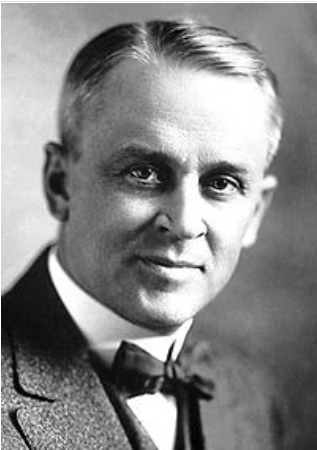
\includegraphics[width=\linewidth]{figures/图1.png}
      \caption{罗伯特·密立根（美国）}
    \end{wrapfigure}

    基本电荷值精确测量者：密立根。
    \begin{itemize}
      \item 密立根利用在电场和重力场中运动的带电油滴精确地测定了基本电荷。
      \item 基本电荷：电荷都是最小基本电荷的整数倍。
    \end{itemize}

    \subsubsection{静态平衡法}
    油滴在平板之间将同时受到重力和静电力的作用。
    
    通过调节板间电压，可以使两个力达到平衡。

    \begin{figure}[H]
      \centering
      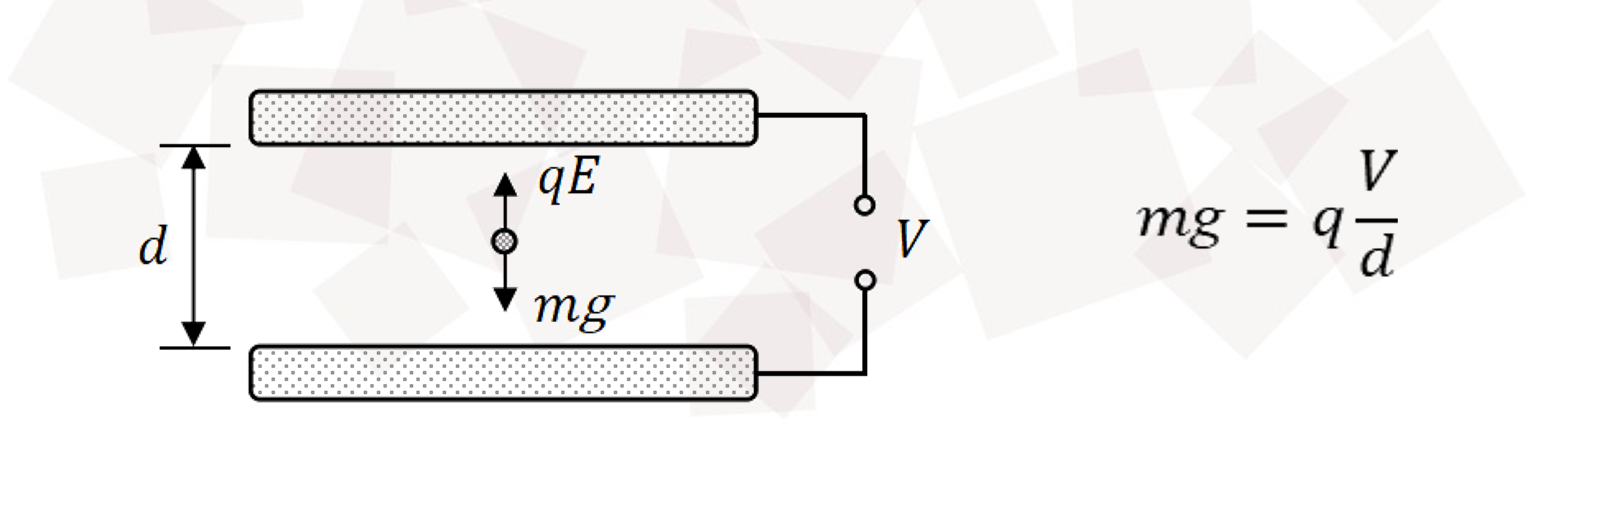
\includegraphics[width=0.75\textwidth]{figures/图2.png}
      \caption{重力与静电力平衡}
    \end{figure}

    \subsubsection{匀速下降法与油滴质量测定}
    设油滴呈小球状，当平板上未加电压时，油滴会加速下落，直到粘滞阻力与重力平衡而匀速下落。

    \[
    \left\{
    \begin{aligned}
    m &= \frac{4}{3}\pi r^3 \rho \\
    f &= 6\pi r\eta v = mg
    \end{aligned}
    \right.
    \quad\Longrightarrow\quad
    r = \sqrt{\frac{9\eta v}{2\rho g}}
    \quad\Longrightarrow\quad
    f = \frac{6\pi r\eta v}{1+\dfrac{b}{pr}}
    \]

    \[
    r
    = \sqrt{
    \frac{9\eta v}{2\rho g}
    \cdot
    \frac{1}{1+\dfrac{b}{pr}}
    }
    \]

    \subsubsection{基本电荷量测定}
    所有带电油滴所携带的电量均是最小电荷量的整数倍，这充分证明了电荷的不连续性。

    \[
    \left.
    \begin{aligned}
    mg &= q\frac{V}{d} \\[1em]
    v &= \frac{l}{t} \\[1em]
    r &= \sqrt{
        \frac{9\eta v}{2\rho g}
        \cdot
        \frac{1}{1+\dfrac{b}{pr}}
    }
    \end{aligned}
    \right\}
    \quad\Longrightarrow\quad
    q = \frac{18\pi}{\sqrt{2\rho g}}
        \left[
            \frac{\eta l}{t\left(1+\dfrac{b}{pr}\right)}
        \right]^{3/2}
        \frac{d}{V}
    \quad\Longrightarrow\quad
    q = mg\frac{d}{V_n} = ne
    \]

    \subsubsection{实验内容}
    主要分为如下两大步骤。
    \begin{enumerate}
      \item 练习找合适油滴
      
      油滴选取原则：应选择电量较小且质量适中的油滴。实验中，通常选取带电量小于10个基本电荷、平衡电压约200V、下落时间在10秒/毫米以内的清晰可见油滴。
      因此，需训练以寻找合适的油滴。若油滴带电量过大，相邻带电油滴将难以区分；若油滴带电量过小，质量也随之减小，更易受空气分子布朗运动的影响。
      
      \item 测量油滴基本电荷量
      \begin{enumerate}
         \item 选取合适油滴，调节电压使油滴悬浮。
         \item 多次测量同一油滴匀速下降的距离及其所用时间（也可使用不同的多颗油滴进行相同的测量）。
         \item 公约数法计算基本电荷量（也可以用其他数据处理方法）。
      \end{enumerate}
    \end{enumerate} 

  \subsection{实验重点（3分）}
  \begin{enumerate}
    \item 了解密立根油滴仪工作特性。
    \item 测定电子基本电荷量。
    \item 掌握密立根油滴实验数据处理方法。
  \end{enumerate}

  \subsection{实验难点（2分）}
  \begin{enumerate}
    \item 选择大小适中、清晰稳定且带电量合适的油滴进行测量；
    \item 准确调节平衡电压，并测量油滴匀速下落的距离和时间；
    \item 根据多次测量数据计算油滴电荷量，利用公约数法确定基本电荷量。
  \end{enumerate}

\section{实验操作与原始数据（50分）}
% 填写自己的实验数据图

\section{结果与分析（30分）}

  \subsection{数据处理与结果（20分）}  
  实验采用静态平衡法测得了多组数据，经软件计算，选取电荷数$n$不超过30，
  且相对误差小于5\%的12组油滴数据，其中多数油滴的电荷数小于10。
  下落距离固定为六格，即$1.5\,\mathrm{mm}$，测量及软件分析结果如表1所示。
  
  \begin{table}[H]
    \centering
    \caption{油滴测量以及软件分析数据}
    \begin{tabular}{ccccccc}
      \toprule
      序号 & 电压值$V/\mathrm{V}$ & 下落时间$t/\mathrm{s}$ & 电荷值$q_i/10^{-19},\,\mathrm{C}$ 
      & 电子数$n$ & 电子电荷值$e_i/10^{-19},\,\mathrm{C}$ & 相对误差 \\
      \midrule
      1 & 165 & 17.68 & 6.59 & 4 & 1.64 & 2.98\% \\
      2 & 193 & 19.82 & 4.71 & 3 & 1.57 & 1.85\% \\
      3 & 113 & 11.56 & 18.6 & 12 & 1.55 & 2.78\% \\
      4 & 70 & 26.81 & 8.08 & 5 & 1.61 & 0.93\% \\
      5 & 127 & 12.56 & 14.6 & 9 & 1.62 & 1.37\% \\
      6 & 156 & 18.56 & 6.46 & 4 & 1.61 & 0.94\% \\
      7 & 238 & 10.26 & 10.6 & 7 & 1.52 & 4.77\% \\
      8 & 77 & 10.01 & 34.2 & 21 & 1.63 & 1.93\% \\
      9 & 69 & 31.07 & 6.49 & 4 & 1.62 & 1.37\% \\
      10 & 88 & 17.13 & 13.0 & 8 & 1.62 & 1.43\% \\
      11 & 61 & 27.01 & 9.17 & 6 & 1.52 & 4.60\% \\
      12 & 104 & 8.78 & 31.1 & 19 & 1.63 & 2.19\% \\
      \bottomrule
    \end{tabular}
  \end{table}

  软件处理的数据仍不够精确，因此我们采用逐差法处理数据，
  即将原始12组电荷量从小到大排列，对相邻两组数据依次逐差，即$\Delta q_i=q_{i+1}-q_i$。
  先估计基本电荷量约为$e_{\text{估}}=1.60\times10^{-19}\,\mathrm{C}$，
  计算$n_i^*=q_i/e_{\text{估}}$并取最近整数$n_i$，再按$e_i=q_i/n_i$计算，例如，
  \[
    \begin{aligned}
      e_1&=\frac{4.71}{3}\times10^{-19}
          =1.57\times10^{-19}\,\mathrm{C} \\[0.5em]
      e_9&=\frac{14.6}{9}\times10^{-19}
          \approx1.62\times10^{-19}\,\mathrm{C}
    \end{aligned}
  \]
  
  逐差结果中，$0.03$和$0.10$明显小于基本电荷量的估计值，说明这几组油滴可能具有相同的电荷数。
  其中微小的电量差异主要来自测量误差，而较大的差值可能对应多个基本电荷，不能直接作为$e$，
  因此需结合全部电量与整数倍关系判断$n_i$，逐差过程中保留原始12组数据。

  其余各组同理，计算结果见表2。表中序号按带电量升序重新排列，末行无相邻后项，故差值为空。

  \begin{table}[H]
    \centering
    \caption{逐差法处理结果}
    \begin{tabular}{cccccc}
      \toprule
      序号 $i$ & $q_i/(10^{-19}\,\mathrm{C})$ & $(q_{i+1}-q_i)/(10^{-19}\,\mathrm{C})$
      & $n_i^*$（计算值） & $n_i$（取整数） & $e_i/(10^{-19}\,\mathrm{C})$ \\
      \midrule
      1 & 4.71 & 1.75 & 2.944 & 3 & 1.57 \\
      2 & 6.46 & 0.03 & 4.038 & 4 & 1.62 \\
      3 & 6.49 & 0.10 & 4.056 & 4 & 1.62 \\
      4 & 6.59 & 1.49 & 4.119 & 4 & 1.65 \\
      5 & 8.08 & 1.09 & 5.050 & 5 & 1.62 \\
      6 & 9.17 & 1.43 & 5.731 & 6 & 1.53 \\
      7 & 10.6 & 2.40 & 6.625 & 7 & 1.51 \\
      8 & 13.0 & 1.60 & 8.125 & 8 & 1.63 \\
      9 & 14.6 & 4.00 & 9.125 & 9 & 1.62 \\
      10 & 18.6 & 12.50 & 11.625 & 12 & 1.55 \\
      11 & 31.1 & 3.10 & 19.438 & 19 & 1.64 \\
      12 & 34.2 & & 21.375 & 21 & 1.63 \\
      \bottomrule
    \end{tabular}
  \end{table}

  各$e_i$及其平均值$\bar e$均保留3位有效数字参与后续计算。
  由上述逐差结果，求得基本电荷量的平均值为
  \[
    \bar e=\frac{1}{12}\sum_{i=1}^{12}e_i
    \approx1.60\times10^{-19}\,\mathrm{C}
  \]

  接下来计算不确定度，由于B类不确定度较为复杂，本实验仅计算A类不确定度，公式为：
  \[
    u_A(\bar e)=\sqrt{\frac{\displaystyle\sum_{i=1}^{N}(e_i-\bar e)^2}{N(N-1)}},
    \qquad N=12
  \]

  各$e_i$为（单位均为$10^{-19}\,\mathrm{C}$）：
  \[
    \begin{aligned}
      e_1&=1.57, & e_2&=1.62, & e_3&=1.62, & e_4&=1.65,\\
      e_5&=1.62, & e_6&=1.53, & e_7&=1.51, & e_8&=1.63,\\
      e_9&=1.62, & e_{10}&=1.55, & e_{11}&=1.64, & e_{12}&=1.63
    \end{aligned}
  \]
  
  将各$e_i$及$\bar e=1.60\times10^{-19}\,\mathrm{C}$代入，得到
  \[
    \begin{aligned}
      u_A(\bar e)
      &=\sqrt{\frac{\begin{gathered}
          (1.57-1.60)^2+(1.62-1.60)^2+(1.62-1.60)^2\\
          {}+(1.65-1.60)^2+(1.62-1.60)^2+(1.53-1.60)^2\\
          {}+(1.51-1.60)^2+(1.63-1.60)^2+(1.62-1.60)^2\\
          {}+(1.55-1.60)^2+(1.64-1.60)^2+(1.63-1.60)^2
        \end{gathered}}{12\times11}}\times10^{-19}\,\mathrm{C}\\[0.5em]
      &=\sqrt{\frac{0.0239}{132}}\times10^{-19}\,\mathrm{C}
      \approx0.0135\times10^{-19}\,\mathrm{C}
      \approx0.01\times10^{-19}\,\mathrm{C}
    \end{aligned}
  \]
  
  因此，实验测得元电荷结果为
  \[
    \boxed{e=(1.60\pm0.01)\times10^{-19}\,\mathrm{C}}
  \]

  \subsection{误差分析（10分）}
  本实验的误差主要来源于以下几个方面：
  \begin{enumerate}
    \item 杂质影响：选取了油滴中的杂质进行测量，杂质和油滴性质完全不同，会使测量结果远偏离正常结果。
    \item 油滴选取：过小的油滴易受布朗运动影响，过大的油滴下落较快，均会增加测量难度，从而增大误差。
    \item 人为计时：启停计时的反应延迟及刻线位置的判断偏差，会影响下落时间测量，尤其在下落较快时相对误差更明显。
    \item 平衡电压：油滴静止状态的判断及电压调节存在偏差，使测得的平衡电压不够准确，油滴缓慢升降时也易被误判为已平衡。
  \end{enumerate}

\section{实验探讨与思考题（10分）}

  \subsection{实验探讨}
  本实验中我明白了，寻找合适油滴需要耐心，也要掌握方法。
  先调好焦距，再结合油滴亮度、下落速度及运动稳定性筛选，可提高测量精度。
  数据处理时，要学会挑选合适的数据，应结合观测记录和测量误差判断数据是否合理，不能仅因结果偏离理论值就将其舍去。

  \subsection{思考题}

    \subsubsection{在测量油滴匀速下降一段距离所花费的时间t时，应选择哪一段最为合适？原因是什么？}
    本实验选取测量范围纵向八格中的中间六格，共$1.5\,\mathrm{mm}$进行计时。
    上下各留一格，便于提前观察油滴、准备启停计时，也为升降和位置调整留出空间。
    六格的距离还能保证适当的计时时长，减小人为反应时间造成的相对误差。

    \subsubsection{什么样的油滴才是合适的待测油滴？该如何挑选呢？可结合自己的实际操作，做一些适当的展开。}
    \begin{enumerate}
      \item 外观清晰：亮度适中、轮廓清楚、近似圆形且孤立，避免误选杂质。
      \item 速度适中：下落较慢，便于计时；也不宜过慢，以免测量过久受扰动。
      \item 大小适当：过小则布朗运动明显，过大则下降过快，均不利于测量。
      \item 带电适中：结合平衡电压判断，便于调节升降；下落慢并不直接代表带电少。
    \end{enumerate}

    \subsubsection{对油滴进行跟踪测量时，有时油滴会逐渐变得模糊，这是为什么呢？应怎样避免在测量过程中丢失油滴？}
    油滴会因空气微流和布朗运动偏离显微镜的焦平面，因此逐渐模糊，此外横向漂移也可能使其离开视野。
    
    实验时应减少振动和气流扰动，选取运动稳定的油滴，适时微调焦距，并利用电压使其升降、保持在视野中部。
    调节动作宜小，持续关注目标，避免与邻近油滴混淆。
    
    此外，油滴蒸发会改变大小与亮度，也可能增大跟踪难度。
    正式测量前应先仔细调焦，并记住目标的位置与亮度；发现其逐渐模糊时，应小幅连续追焦，避免大幅调节或频繁切换观察目标。

    \subsubsection{尝试用其他数据处理方式，处理数据，计算基本电荷量。}
    \begingroup
    \setlength{\intextsep}{8pt}
    除原逐差法外，还可采用平均值法、多重差值法及作图拟合法进行数据处理，各方法所得$e$均保留3位有效数字。

    \noindent{\CJKfontspec[AutoFakeBold=2.5]{SimSun}\bfseries （1）平均值法}\par
    先保留原始12组电量，从小到大排列并作相邻差值，结合整数倍关系确定电荷数$n$，
    这一步与表2相同。随后将电荷数相同的电量取平均，计算$e_n=\bar q_n/n$，最后对各类$e_n$取平均，即
    \[
      \bar q_4=\frac{6.46+6.49+6.59}{3}\times10^{-19}
      \approx6.51\times10^{-19}\,\mathrm{C},\qquad
      e_4=\frac{\bar q_4}{4}\approx1.63\times10^{-19}\,\mathrm{C}.
    \]

    因此12组原始数据归为10类，结果见表3。

    \begin{table}[H]
      \centering
      \caption{平均值法处理结果}
      \begin{tabular}{ccc}
        \toprule
        电荷数$n$ & $\bar q_n/(10^{-19}\,\mathrm{C})$ & $e_n/(10^{-19}\,\mathrm{C})$ \\
        \midrule
        3 & 4.71 & 1.57 \\
        4 & 6.51 & 1.63 \\
        5 & 8.08 & 1.62 \\
        6 & 9.17 & 1.53 \\
        7 & 10.6 & 1.51 \\
        8 & 13.0 & 1.63 \\
        9 & 14.6 & 1.62 \\
        12 & 18.6 & 1.55 \\
        19 & 31.1 & 1.64 \\
        21 & 34.2 & 1.63 \\
        \bottomrule
      \end{tabular}
    \end{table}
    将10类$e_n$取平均，得$e_{\text{均值}}=\frac{1}{10}\sum_n e_n=1.59\times10^{-19}\,\mathrm{C}$。

    \noindent{\CJKfontspec[AutoFakeBold=2.5]{SimSun}\bfseries （2）多重差值法}\par
    保留原始12组电量，排序后计算$\Delta q_i=q_{i+1}-q_i$，再计算
    $\Delta^2q_i=\Delta q_{i+1}-\Delta q_i=q_{i+2}-2q_{i+1}+q_i$。
    表4列出一阶差值及二阶差值的绝对值，选取$\Delta n_i=1$的一阶项与$|\Delta^2n_i|=1$的二阶项并加粗，
    它们在$q_i\approx n_i e$关系下对应一个基本电荷。

    \begin{table}[H]
      \centering
      \caption{多重差值法处理结果（电荷量单位：$10^{-19}\,\mathrm{C}$）}
      \small
      \begin{tabular}{ccccc}
        \toprule
        序号 $i$ & $q_i$ & $n_i$ & $\Delta q_i$ & $|\Delta^2 q_i|$ \\
        \midrule
        1 & 4.71 & 3 & $\mathbf{1.75}$ & $\mathbf{1.72}$ \\
        2 & 6.46 & 4 & 0.03 & 0.07 \\
        3 & 6.49 & 4 & 0.10 & $\mathbf{1.39}$ \\
        4 & 6.59 & 4 & $\mathbf{1.49}$ & 0.40 \\
        5 & 8.08 & 5 & $\mathbf{1.09}$ & 0.34 \\
        6 & 9.17 & 6 & $\mathbf{1.43}$ & 0.97 \\
        7 & 10.6 & 7 & $\mathbf{2.40}$ & 0.80 \\
        8 & 13.0 & 8 & $\mathbf{1.60}$ & 2.40 \\
        9 & 14.6 & 9 & 4.00 & 8.50 \\
        10 & 18.6 & 12 & 12.50 & 9.40 \\
        11 & 31.1 & 19 & 3.10 & \\
        12 & 34.2 & 21 & & \\
        \bottomrule
      \end{tabular}
    \end{table}

    将8个加粗数据平均，得$e_{\text{多差}}=1.61\times10^{-19}\,\mathrm{C}$。
    本实验算至二阶，考虑到更高阶差分可能会放大测量误差。

    \noindent{\CJKfontspec[AutoFakeBold=2.5]{SimSun}\bfseries （3）作图拟合法}\par
    对原始12组数据作$q$--$n$图，按$q=en$进行等权、过原点最小二乘拟合，得到
    \[
      e_{\text{拟合}}=\frac{\sum_{i=1}^{12}n_iq_i}{\sum_{i=1}^{12}n_i^2}
      \approx1.61\times10^{-19}\,\mathrm{C},\qquad R^2=0.9984
    \]

    \begin{figure}[H]
      \centering
      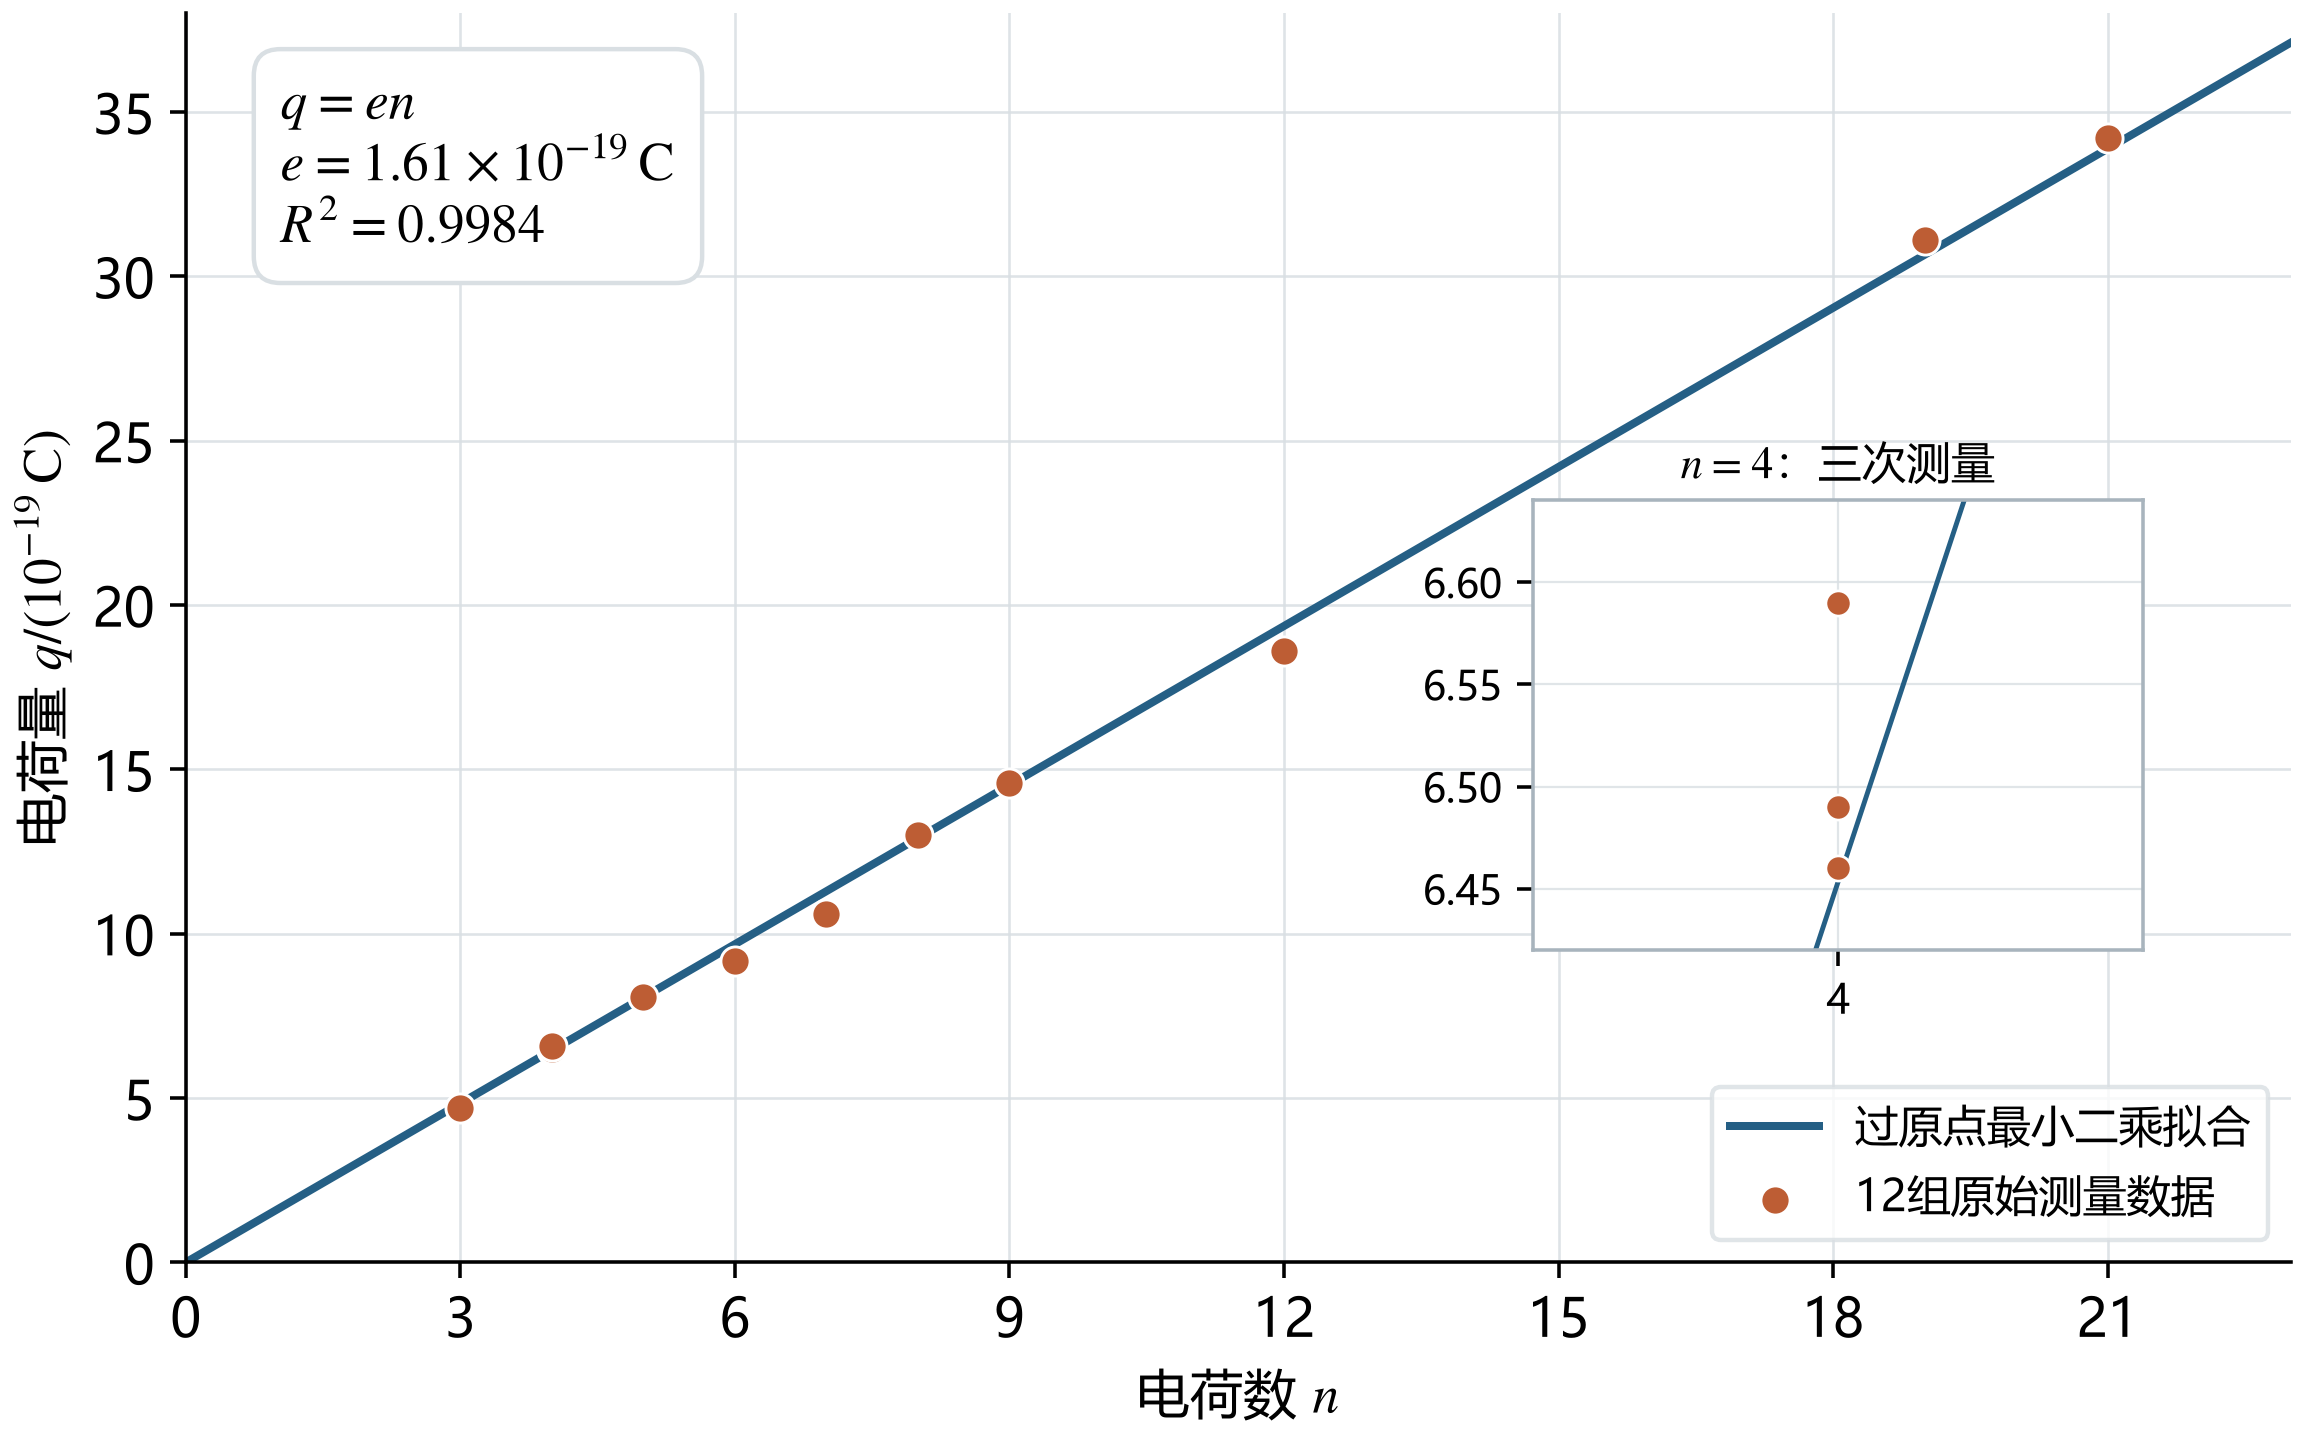
\includegraphics[width=0.6\textwidth]{figures/图5.png}
      \caption{作图拟合法处理结果}
    \end{figure}

    \noindent{\CJKfontspec[AutoFakeBold=2.5]{SimSun}\bfseries （4）结果比较}\par
    以$e_0=1.602\times10^{-19}\,\mathrm{C}$为参考值，
    按各方法保留3位有效数字的结果计算相对误差$\delta=|e-e_0|/e_0\times100\%$，比较优缺点如下。
    \begin{table}[H]
      \centering
      \caption{四种数据处理方法比较}
      {\small
      \setlength{\tabcolsep}{4pt}
      \begin{tabular}{ccccc}
        \toprule
        方法 & $e/(10^{-19}\,\mathrm{C})$ & 相对误差 & 优点 & 局限 \\
        \midrule
        逐差法 & 1.60 & 0.12\% & 逐差辅助判定电荷数，计算直观 & 依赖$n$的判定，未考虑各组精度差异 \\
        平均值法 & 1.59 & 0.75\% & 计算简单，同电荷数组等权 & 依赖$n$的判定，未考虑各组精度差异 \\
        多重差值法 & 1.61 & 0.50\% & 利用不同阶差值估计$e$ & 差值相关且选项依赖$n$ \\
        作图拟合法 & 1.61 & 0.50\% & 直观反映整体关系 & 强制过原点，大$n$点影响较大 \\
        \bottomrule
      \end{tabular}
      }
    \end{table}

    逐差法与平均值法分别对12组测量和10类电荷数等权平均，权重不同，故结果略有差异。
    多重差值法与拟合法修约后结果相同。各法共用$n$的判定，不能以结果接近作为$n$正确的独立证据，
    方法优劣也不能仅凭相对误差判断，需根据情况灵活采用合适方法。
    \endgroup

\vspace*{\fill} % 使下面内容在页面底部显示
\noindent
\begin{minipage}{\textwidth}
  注意事项：

  \begingroup
    \setlength{\leftskip}{2em} % 1--4整体向右缩进两个汉字宽度
    1. 用PDF格式上传“实验报告”，文件名：学生姓名+学号+实验名称+周次。

    2. “实验报告”必须递交在“学在浙大”本课程内对应实验项目的“作业”模块内。

    3. “实验报告”成绩必须在“浙江大学物理实验教学中心网站”-“选课系统”内查询。

    4. 教学评价必须在“浙江大学物理实验教学中心网站”-“选课系统”内进行，学生必须进行教学评价，才能看到实验报告成绩，教学评价须在本次实验结束之后3天内进行。\par
  \endgroup

  \begin{center}
    {\CJKfontspec[AutoFakeBold=2.5]{SimSun}\bfseries 浙江大学物理实验教学中心制}
  \end{center}
\end{minipage}

\end{document}

